
\begin{frame}{An application in molecular dynamics simulation (MDS)}
\begin{columns}
\begin{column}{0.5\textwidth}
\begin{itemize}
    \item Given a molecule consisting of $N_a$ atoms, simulate $T$ timesteps of molecular motion to generate data $\mathcal D \in \mathbb R^{T \times 3N_a}$
    \item These samples concentrate near a low-dimensional manifold which we can estimate using ML
\end{itemize}
\end{column}
\begin{column}{0.5\textwidth}
\begin{figure}
    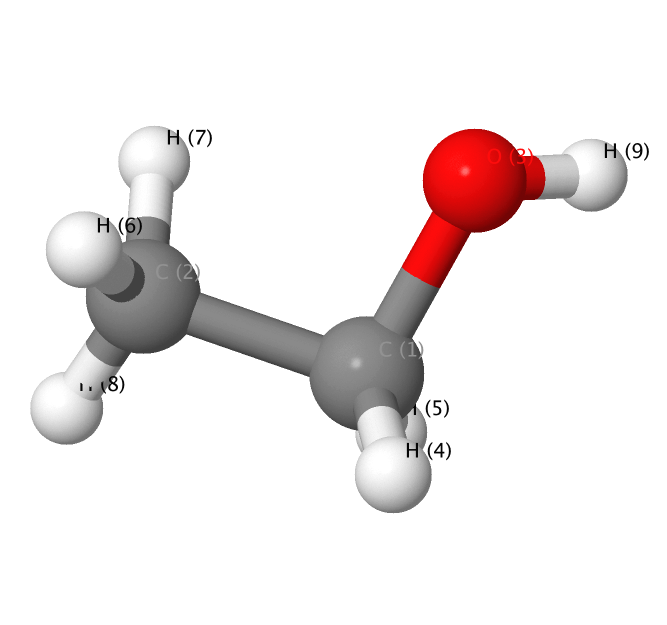
\includegraphics[width=4cm]{img/ethanol.png}
    \caption*{Ethanol ($N_a = 9$) \parencite{Chmiela2018-at}}
\end{figure}
\end{column}
\end{columns}
\end{frame}
 % {\it shape space} of $N_a$ atoms in $3$ dimensions $\Sigma_{3}^{N_a} = \mathbb R^{3N_a} / E(3)$, where $E(3)$ is the three-dimensional Euclidean group of rotations and translations
\begin{frame}[fragile]{Representing invariant geometry}
\begin{columns}
\begin{column}{0.5\textwidth}
\begin{itemize}
    \item We featurize each configuration using planar angles prior to ML \parencite{chen2019modern}
\end{itemize}
\begin{figure}
\begin{tikzcd}
\mathbb R^{3N_a} & \mathbb R^{3 { N_a \choose 3}} & \mathbb R^M \\
\mathcal M \arrow[r, "\alpha"] \arrow[u,  symbol=\subset] & \alpha(\mathcal M)\arrow[r, "\phi"] \arrow[u,  symbol=\subset] & \phi(\alpha(\mathcal M)) \arrow[u,  symbol=\subset] 
\end{tikzcd}
\caption*{$\alpha$ is the planar angle map}
\end{figure}
\end{column}
\begin{column}{0.4\textwidth}
\begin{figure}
    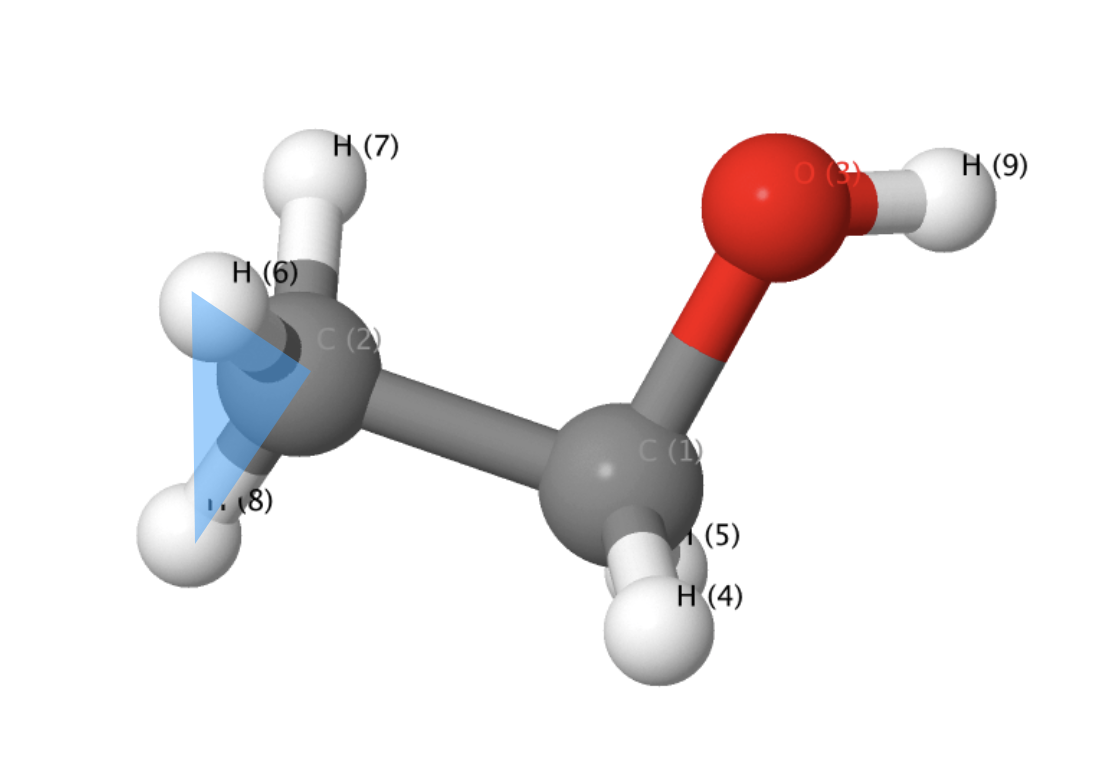
\includegraphics[width=4cm]{img/planar.png}
    \caption*{Planar angles are formed by triplets of atoms}
\end{figure}
\end{column}
\end{columns}
\end{frame}

\begin{frame}[fragile]{The learned manifold}
\vspace{-2cm}
\begin{figure}
    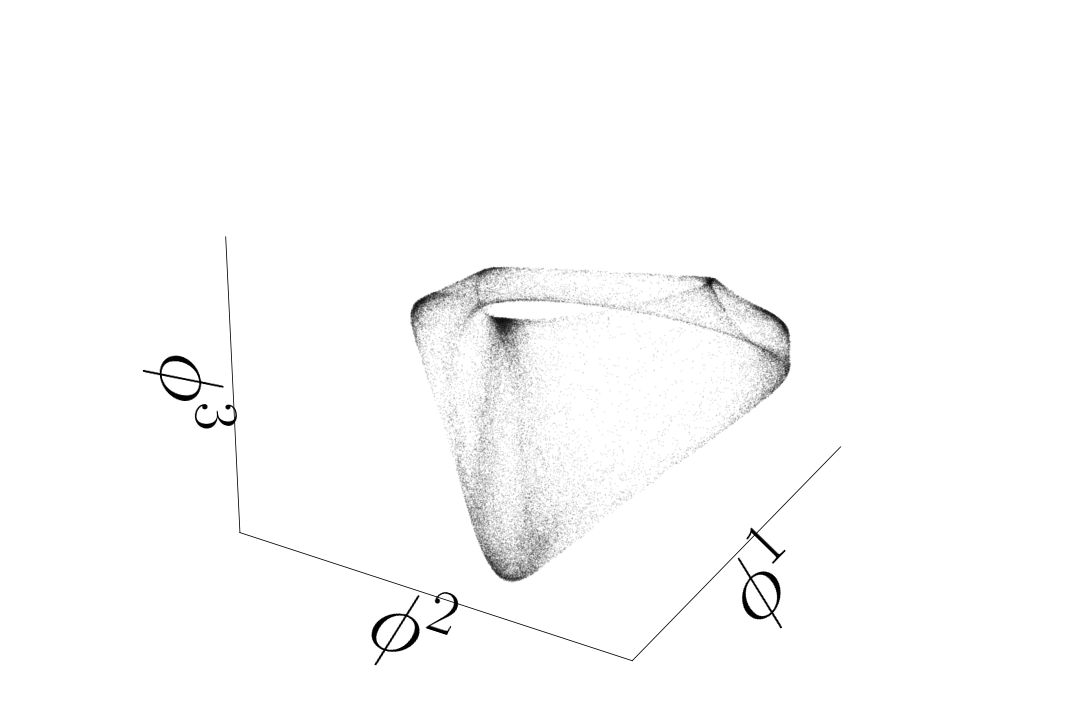
\includegraphics[width=10cm]{img/ethanol_embedding.png}
    \caption*{Diffusion Maps embedding of $T = 50000$ ethanol configurations into $M=3$ dimensions shows a $2$ dimensional toroidal molecular manifold}
\end{figure}
\end{frame}

\begin{frame}{Visually interpreting embeddings}
\vspace{-.5cm}
\begin{figure}[!htp]
    \centering
    \begin{tabular}{cc}
        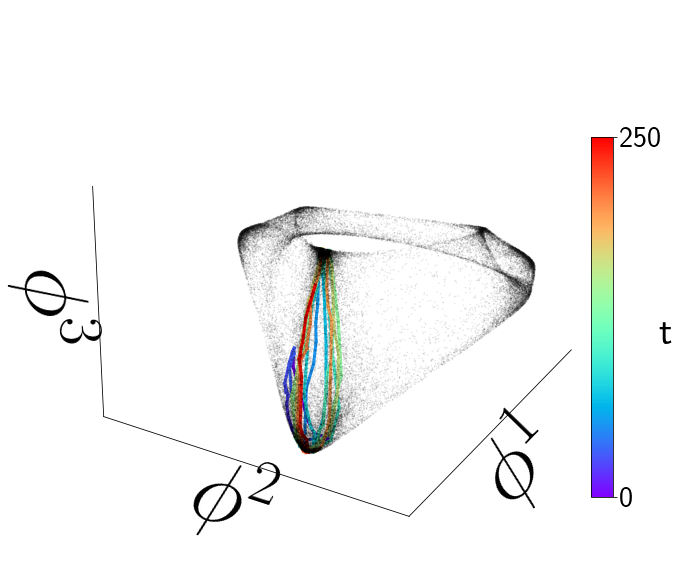
\includegraphics[width=0.35\textwidth]{img/ethanol_trajectory.png} &
        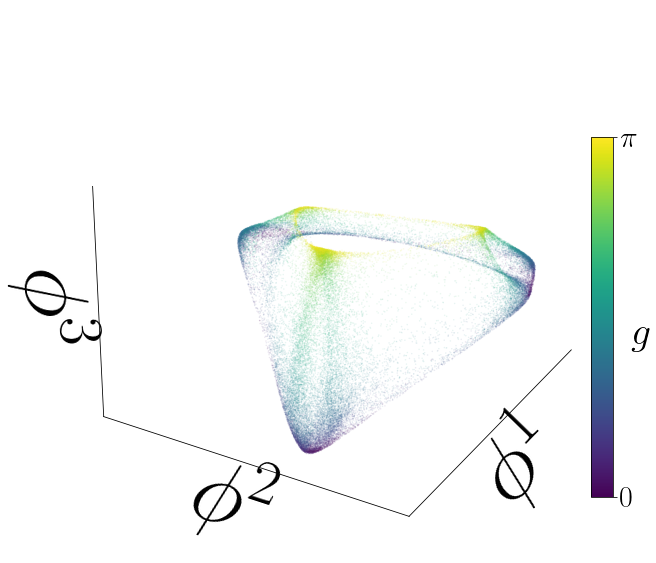
\includegraphics[width=0.35\textwidth]{img/ethanol_color.png} \\
        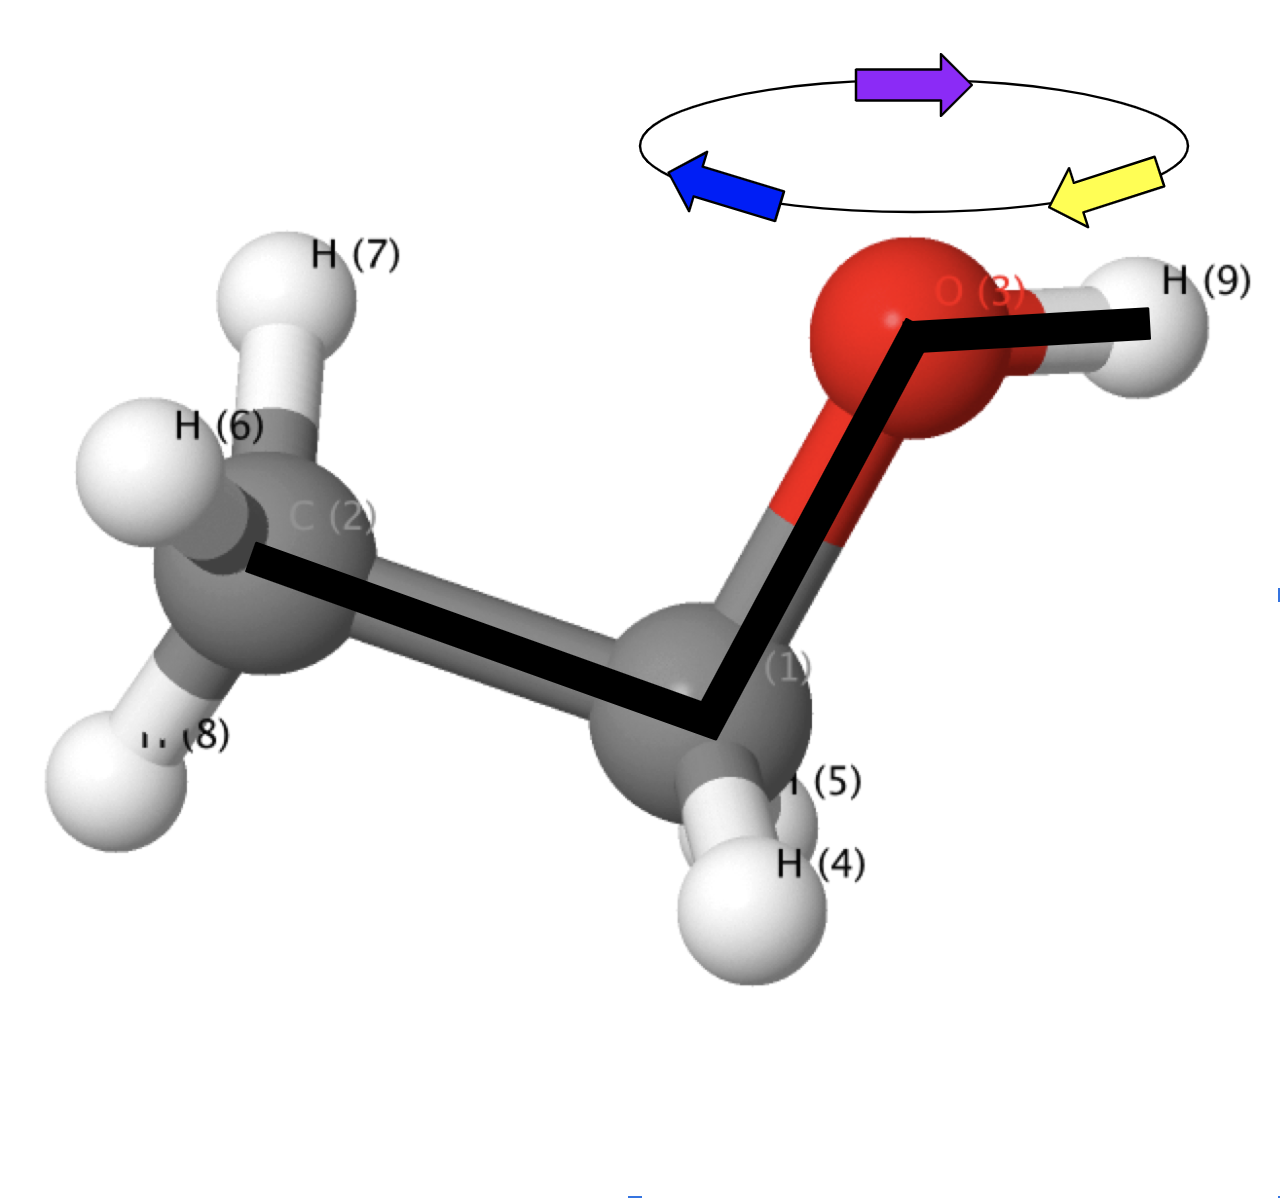
\includegraphics[width=0.3\textwidth]{img/ethanol_dynamics.png} & \vspace{1cm} 
        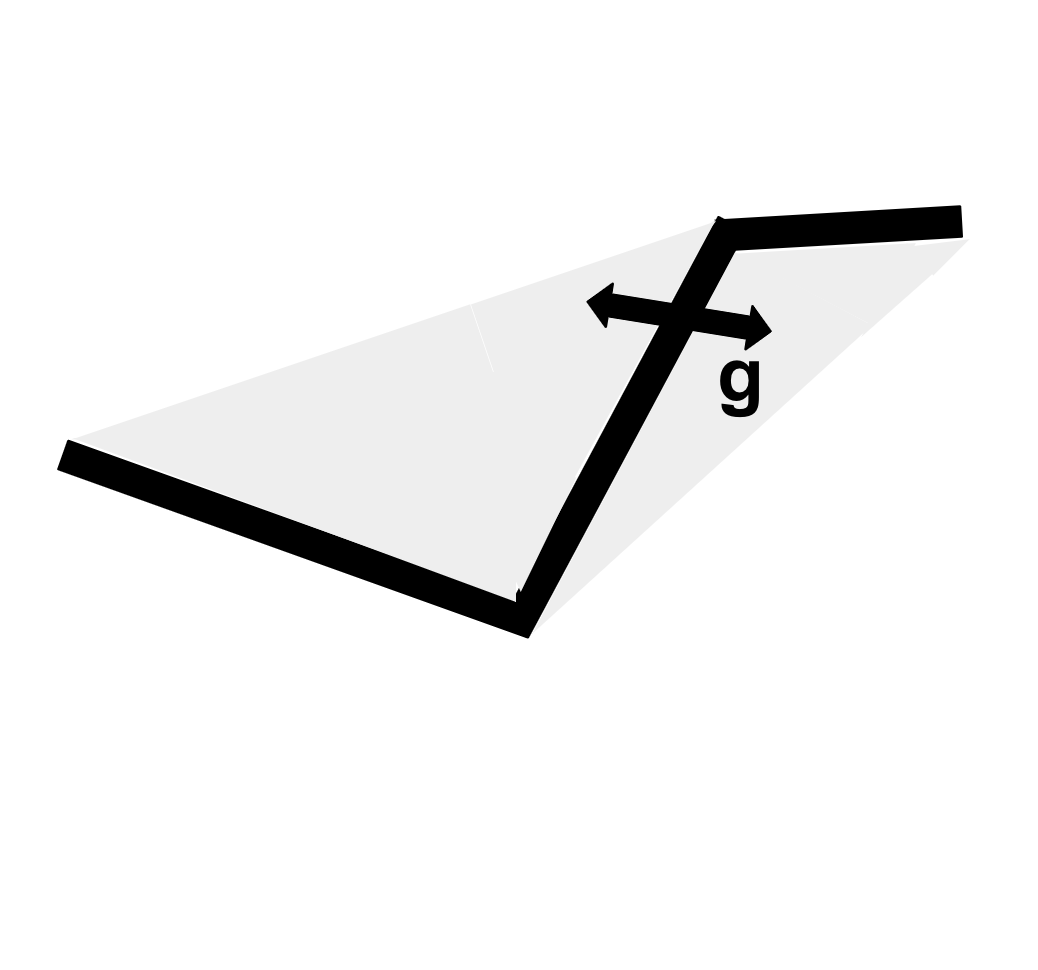
\includegraphics[width=0.25\textwidth]{img/torsion_square.png}
    \end{tabular}
    \vspace{-2cm}
    \caption*{Movement in the ethanol simulation corresponds to hydroxyl rotation}
\end{figure}
\end{frame}

\begin{frame}{Interpretability is important}
\begin{itemize}
\item Mechanistic understanding
\item Generative control 
\item Statistical efficiency
\end{itemize}
\end{frame}

\begin{frame}{Scaling interpretability}
\begin{figure}[!htp]
    \centering
    \begin{tabular}{p{2.5cm}p{2.5cm}p{2.5cm}p{2.5cm}}
        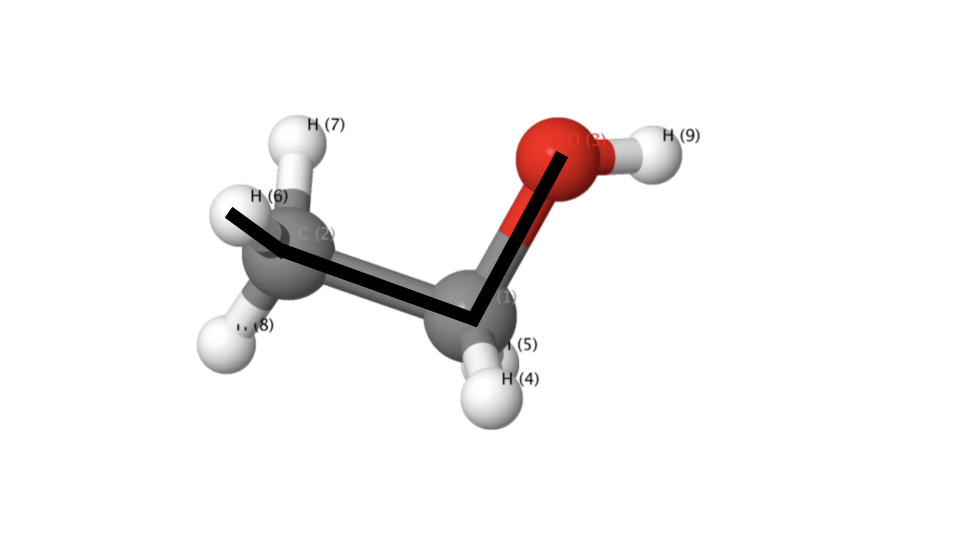
\includegraphics[width=0.25\textwidth, trim={2cm 3cm 5cm 0cm}, clip]{img/ethanol_g0.png} &
        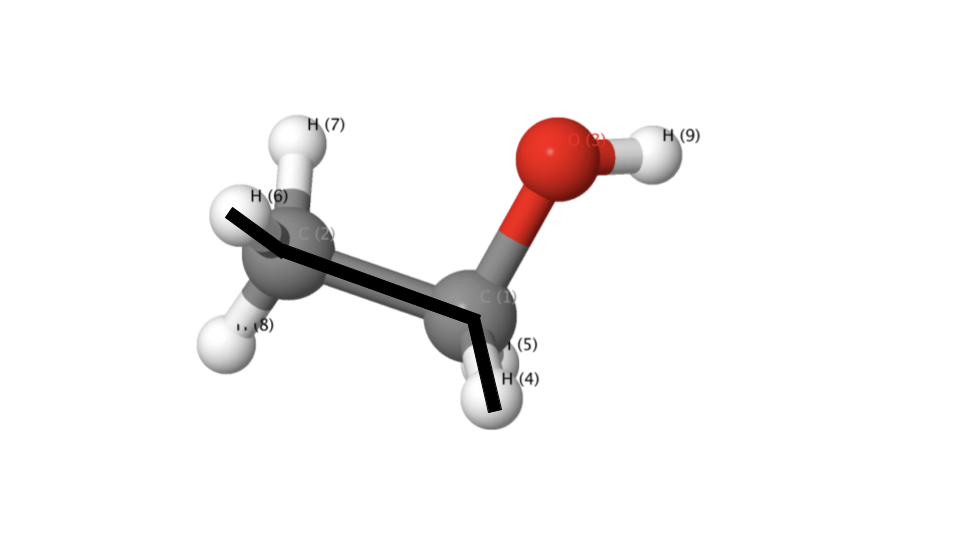
\includegraphics[width=0.25\textwidth, trim={2cm 3cm 5cm 0cm}, clip]{img/ethanol_g1.png} &
          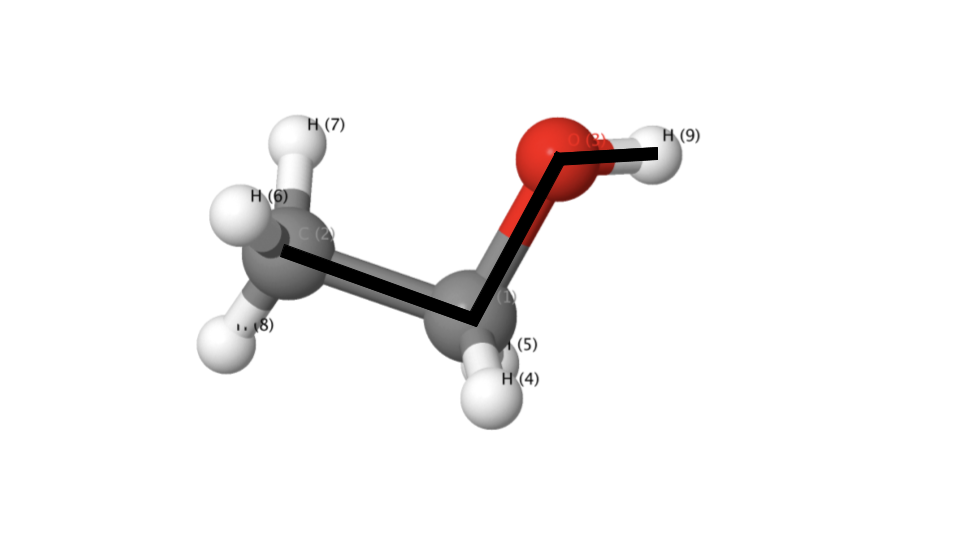
\includegraphics[width=0.25\textwidth, trim={2cm 3cm 5cm 0cm}, clip]{img/ethanol_g2.png} &
          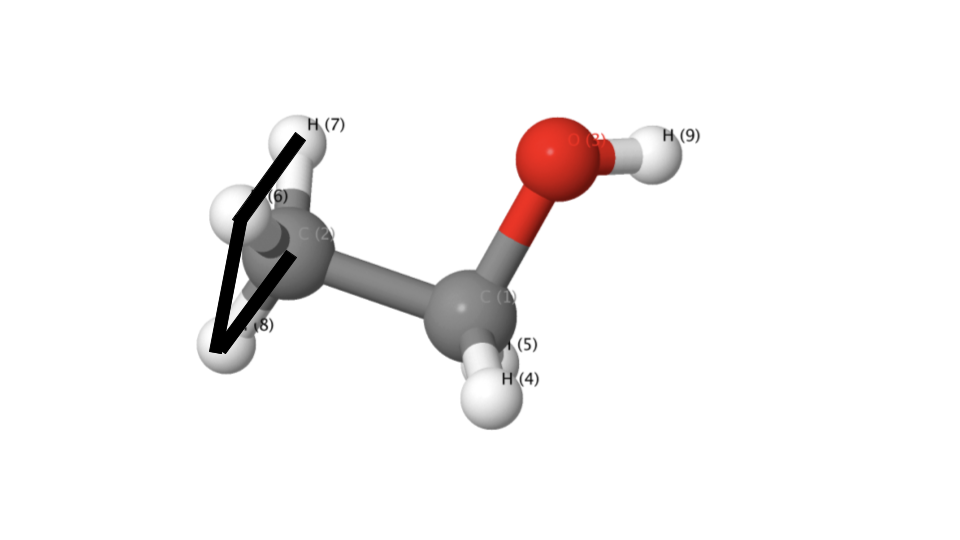
\includegraphics[width=0.25\textwidth, trim={2cm 3cm 5cm 0cm}, clip]{img/ethanol_g3.png}  \\
        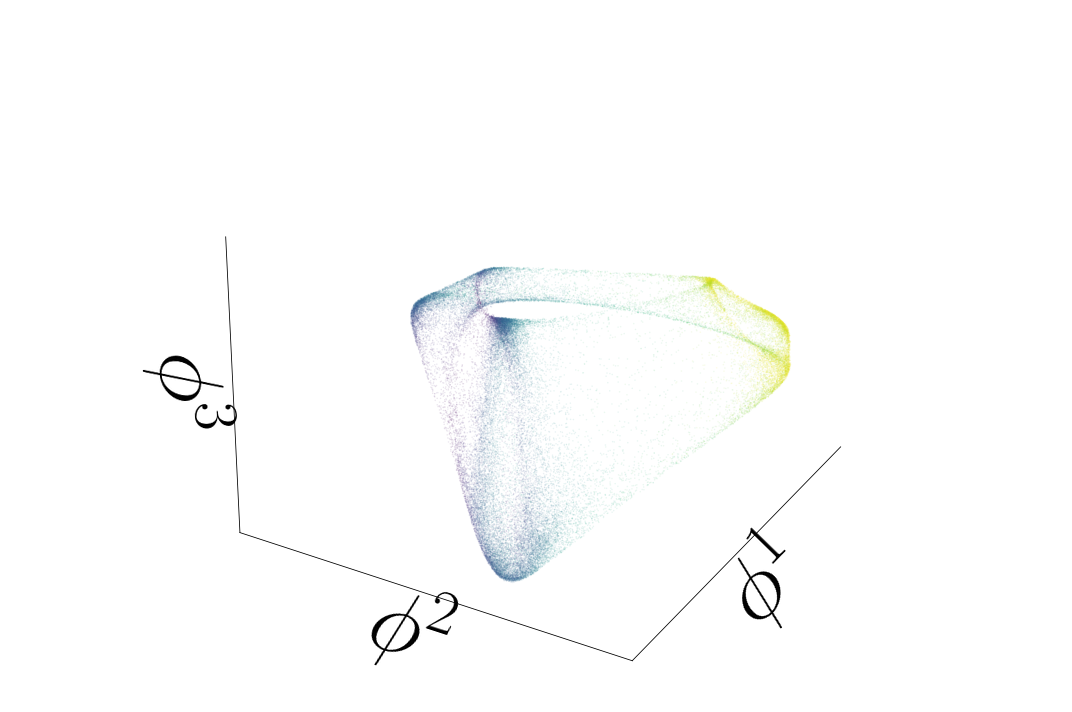
\includegraphics[width=0.25\textwidth, trim={1cm 0cm 4cm 4cm}, clip]{img/ethanol_embedding_0.png} &
        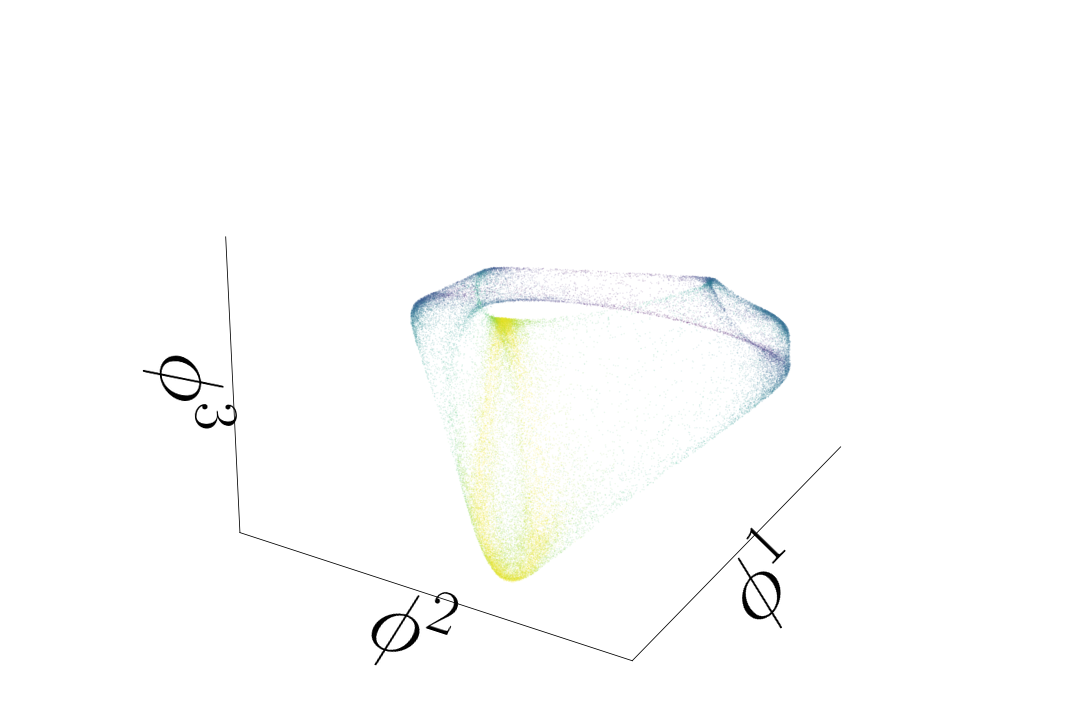
\includegraphics[width=0.25\textwidth, trim={1cm 0cm 4cm 4cm}, clip]{img/ethanol_embedding_1.png} &
         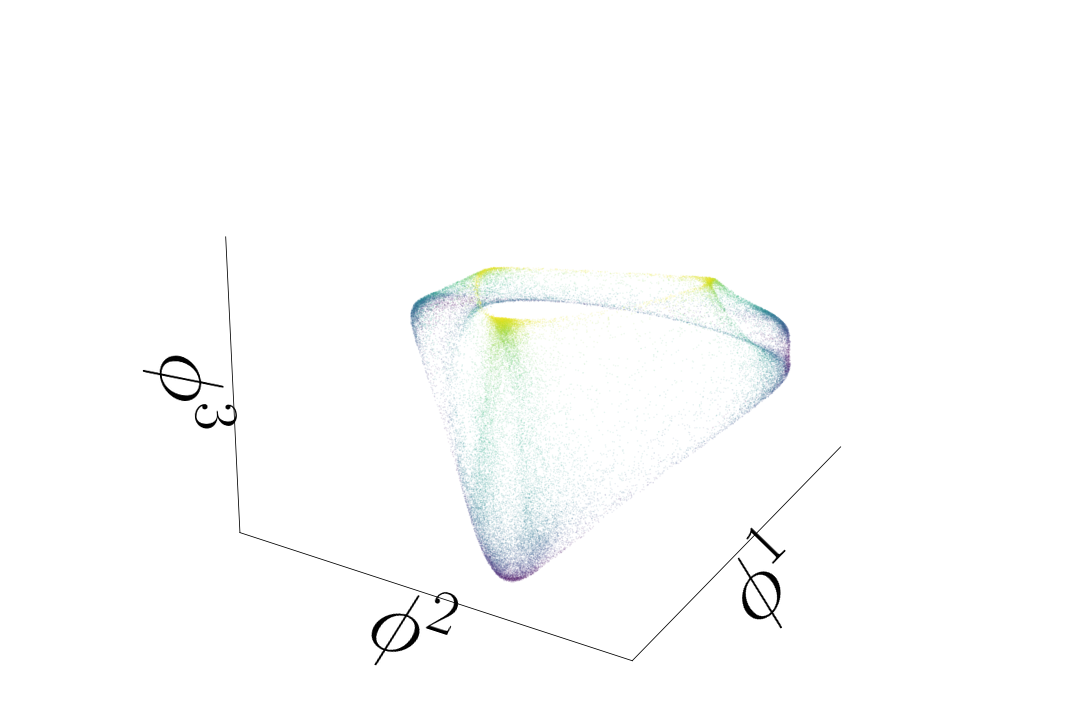
\includegraphics[width=0.25\textwidth, trim={1cm 0cm 4cm 4cm}, clip]{img/ethanol_embedding_2.png}  &
          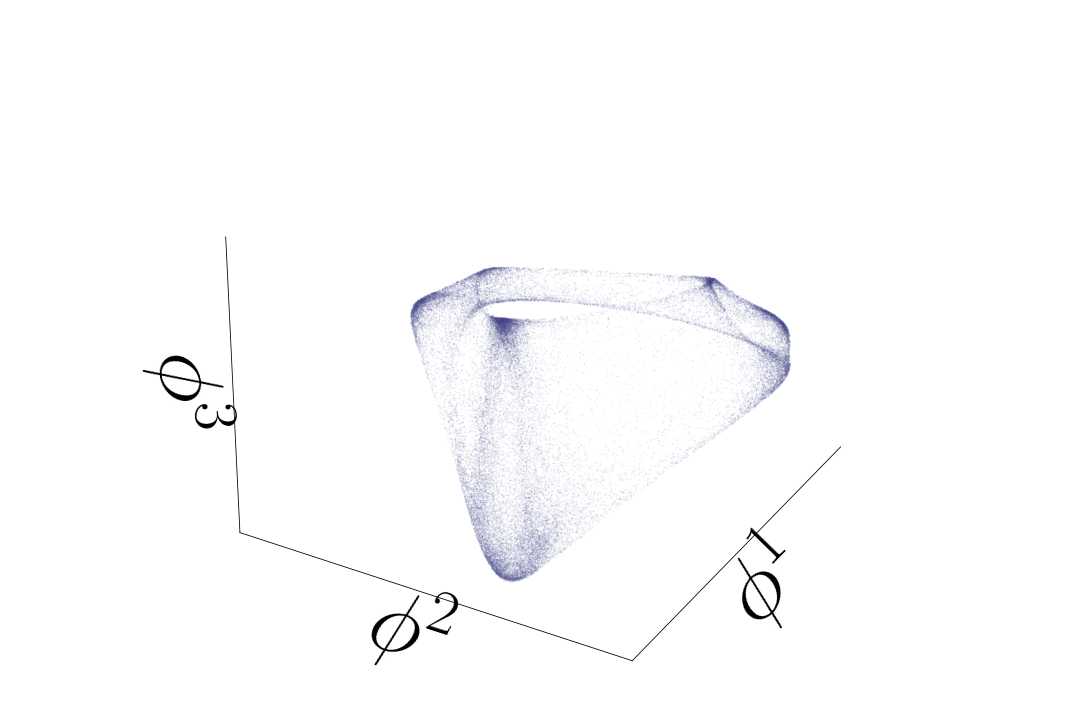
\includegraphics[width=0.25\textwidth, trim={1cm 0cm 4cm 4cm}, clip]{img/ethanol_embedding_3.png} 
    \end{tabular}
    %\vspace{-2cm}
    \caption*{$4$ of the $756$ bond torsions in ethanol}
\end{figure}



\end{frame}

\begin{frame}{Explanations}
\begin{definition}[Explanation]
    $D$ functions $g^p$ form a {\it explanation} if their gradients form rank $D$ linear maps from $\mathbb R^D \to \mathbb R^D$.
\end{definition}
\begin{figure}[!htp]
\tiny
    \centering
    \begin{tabular}{p{2cm}p{2cm}p{2cm}p{2cm}}
        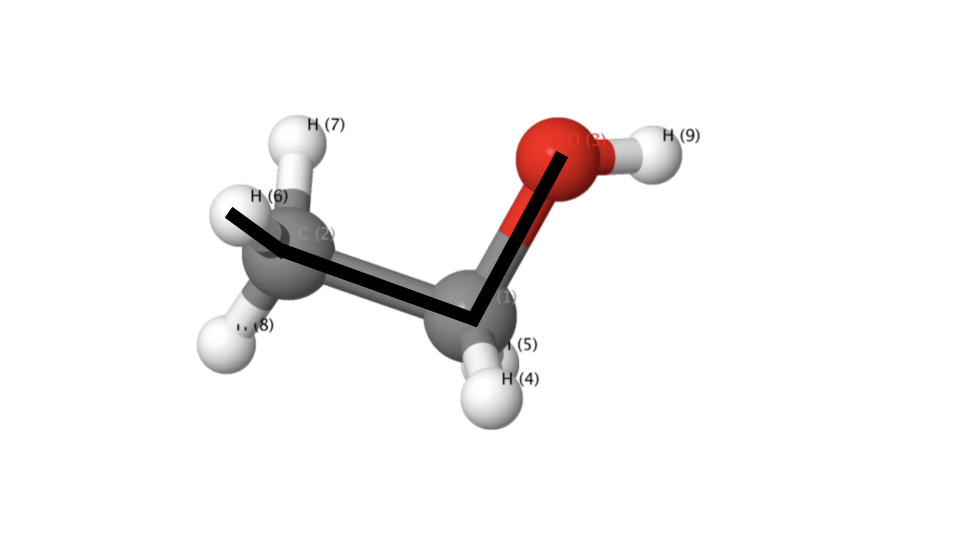
\includegraphics[width=0.2\textwidth, trim={2cm 3cm 5cm 0cm}, clip]{img/ethanol_g0.png} &
        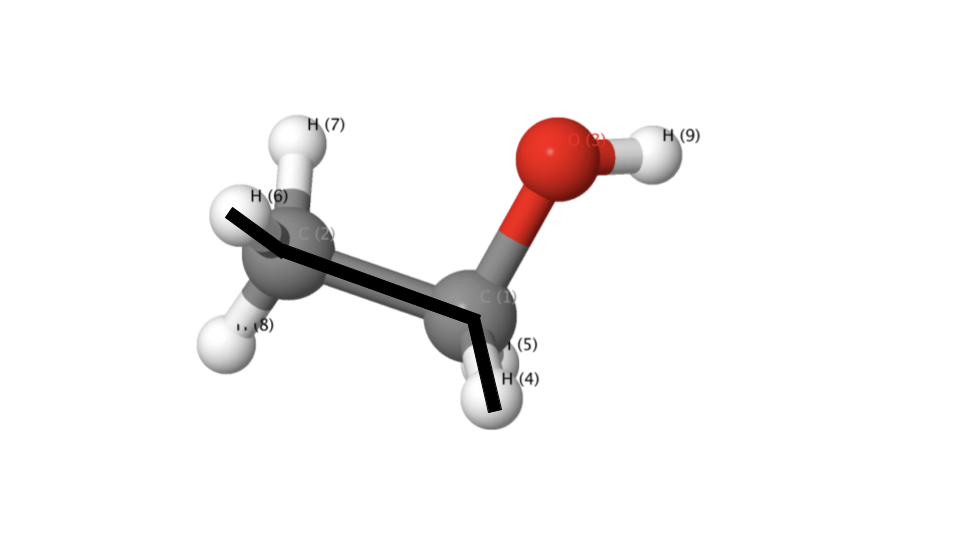
\includegraphics[width=0.2\textwidth, trim={2cm 3cm 5cm 0cm}, clip]{img/ethanol_g1.png} &
          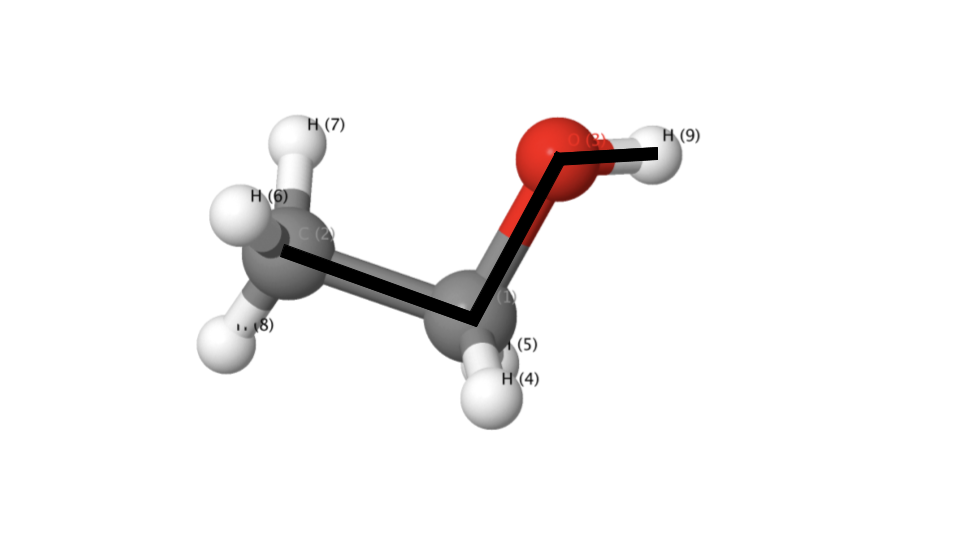
\includegraphics[width=0.2\textwidth, trim={2cm 3cm 5cm 0cm}, clip]{img/ethanol_g2.png} &
          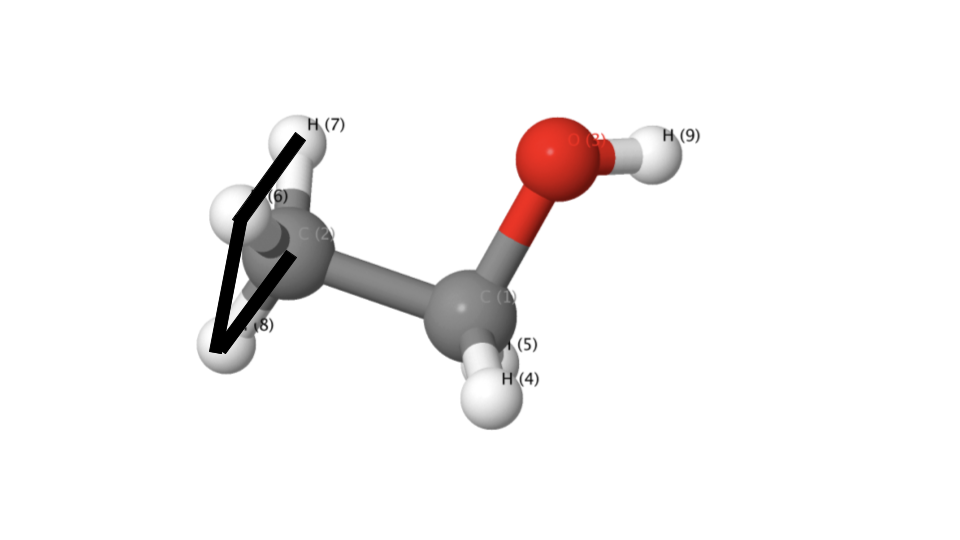
\includegraphics[width=0.2\textwidth, trim={2cm 3cm 5cm 0cm}, clip]{img/ethanol_g3.png}  \\
        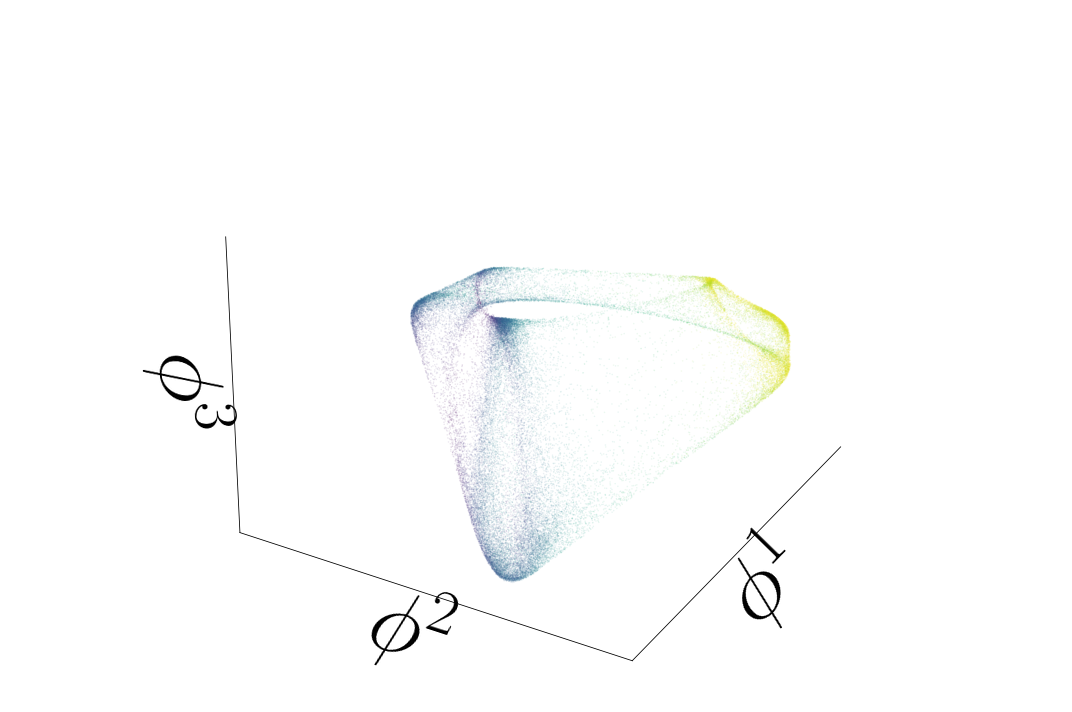
\includegraphics[width=0.2\textwidth, trim={1cm 0cm 4cm 4cm}, clip]{img/ethanol_embedding_0.png} &
        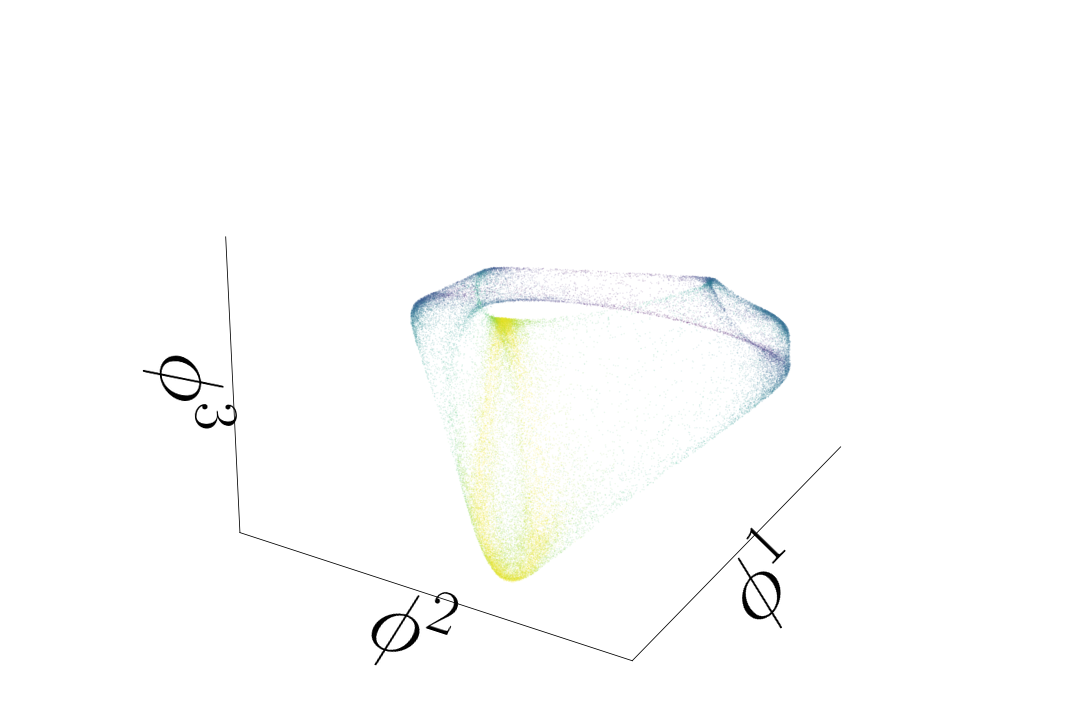
\includegraphics[width=0.2\textwidth, trim={1cm 0cm 4cm 4cm}, clip]{img/ethanol_embedding_1.png} &
         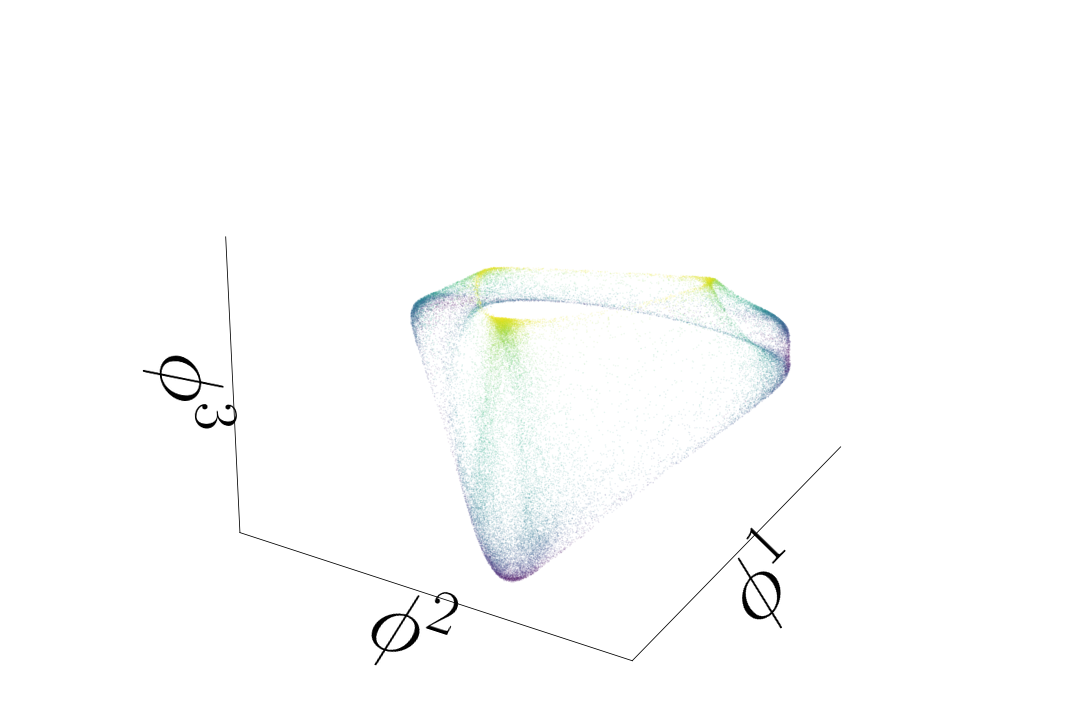
\includegraphics[width=0.2\textwidth, trim={1cm 0cm 4cm 4cm}, clip]{img/ethanol_embedding_2.png}  &
          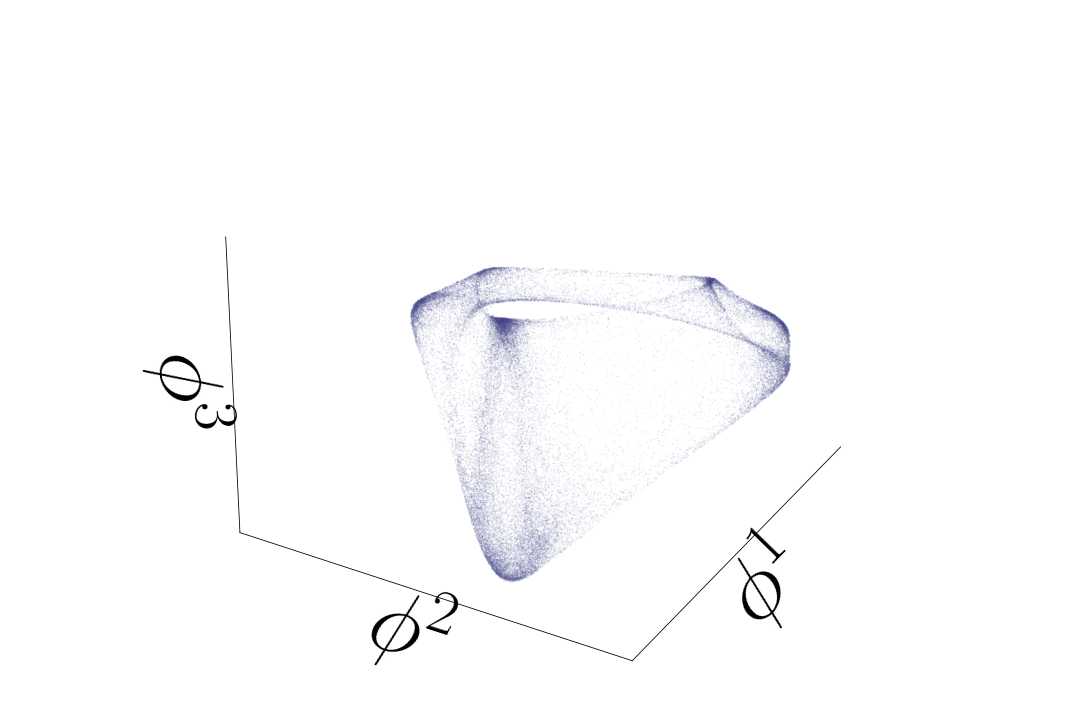
\includegraphics[width=0.2\textwidth, trim={1cm 0cm 4cm 4cm}, clip]{img/ethanol_embedding_3.png} \\
          \centering $g^1$ & \centering  $g^2$ & \centering  $g^3$ & \centering  $g^4$
    \end{tabular}
    %\vspace{-2cm}
\end{figure}
\begin{table}[htbp]
\tiny
    \centering
    \begin{tabular}{|c|c|c|c|c|}
        \hline
        & \( g^1 \) & \( g^2 \) & \( g^3 \) & \( g^4 \) \\
        \hline
        \( g^1 \) & \( x \) & \( x \) &\checkmark & \( x \) \\
        \hline
        \( g^2 \) & \( x \) & \( x \) & \checkmark  & \( x \) \\
        \hline
        \( g^3 \) & \checkmark & \checkmark & \( x \) & \( x \) \\
        \hline
        \( g^4 \) & \( x \) & \( x \) & \( x \) &\( x \) \\
        \hline
    \end{tabular}
    \caption*{Are these explanations?}
    \label{tab:4x4table}
\end{table}
\end{frame}

\begin{frame}[fragile]{Interpretability examples}
\centering
\begin{figure}[H]
    \centering
\begin{tikzcd}[column sep=small]
 & \text{Data } \mathcal{D} \in  \mathbb R^{N \times B} \arrow[dl] \arrow[dr] & \\
\text{Embedding } \phi(\mathcal{D}) & &  \text{Dictionary } g (\mathcal D) = [g^1, \dots, g^P]
\end{tikzcd}
    \label{fig:summary}
\end{figure}
\begin{table}[H]
\tiny
\centering
\begin{tabular}{|p{1.8cm}|p{1.8cm}|p{2cm}|p{2.4cm}|p{2cm}|}
\hline
\textbf{Data} & \textbf{Featurization} &\textbf{Embedding} & \textbf{Dictionary} & \textbf{Explanation} \\
\hline
Configurations & Planar angles & UMAP & Dihedral angles & Methyl rotation \\
Sentences & Tokens & LLM embeddings & Sparse autoencoder & Time of day \\
Cells & Gene expression & UMAP & Gene sets & Cell cycle \\
Galaxies & Spectra & Diffusion maps & Stellar features & Age \\
\hline
\end{tabular}
\label{tab:concept_examples}
\caption*{Examples of explanations in various scientific domains}
\end{table}
\end{frame}


\begin{frame}{Problem statement}
\begin{itemize}
\item Our goal: find $D$ function subset of $g$ whose gradients w.r.t. $\mathcal M$ form a rank $D$ matrix almost everywhere
\end{itemize}
\begin{proposition}[Cut-locus theorem \parencite{Sheng2009-ij}]
Every manifold $\M$ has an explanation defined everywhere except for a singular set.
\end{proposition}
\begin{itemize}
    % \item Note: this will not necessarily be a bijection (show sin wave) - for this reason we call the recovered rank $d$ set an {\it explanation}
    \item \cite{Koelle2022-oj}: Provide a sparse regression estimator for selecting explanations w.r.t. $\phi$
    \item \cite{Koelle2024-no}: Select explanations without $\phi$
\end{itemize}
\end{frame}

